\documentclass{article}
\usepackage{lscape}
\usepackage{gensymb}
\usepackage{textcomp}
\usepackage{multicol}
\usepackage[version=3]{mhchem} % Package for chemical equation typesetting
\usepackage{siunitx} % Provides the \SI{}{} and \si{} command for typesetting SI units
\usepackage{graphicx} % Required for the inclusion of images
\usepackage{natbib} % Required to change bibliography style to APA
\usepackage{amsmath} % Required for some math elements 
\usepackage{hyperref}
\usepackage[a4paper,margin=0.5in]{geometry}
\setlength\parindent{0pt} % Removes all indentation from paragraphs

\renewcommand{\labelenumi}{\alph{enumi}.} % Make numbering in the enumerate environment by letter rather than
\usepackage[a4paper,margin=0.5in]{geometry}
\begin{document}
	\title{Literature Review}
	\author{Philipp Duernay}
	\maketitle

	\section{Single Shot Detectors}
	\begin{figure}[h]
		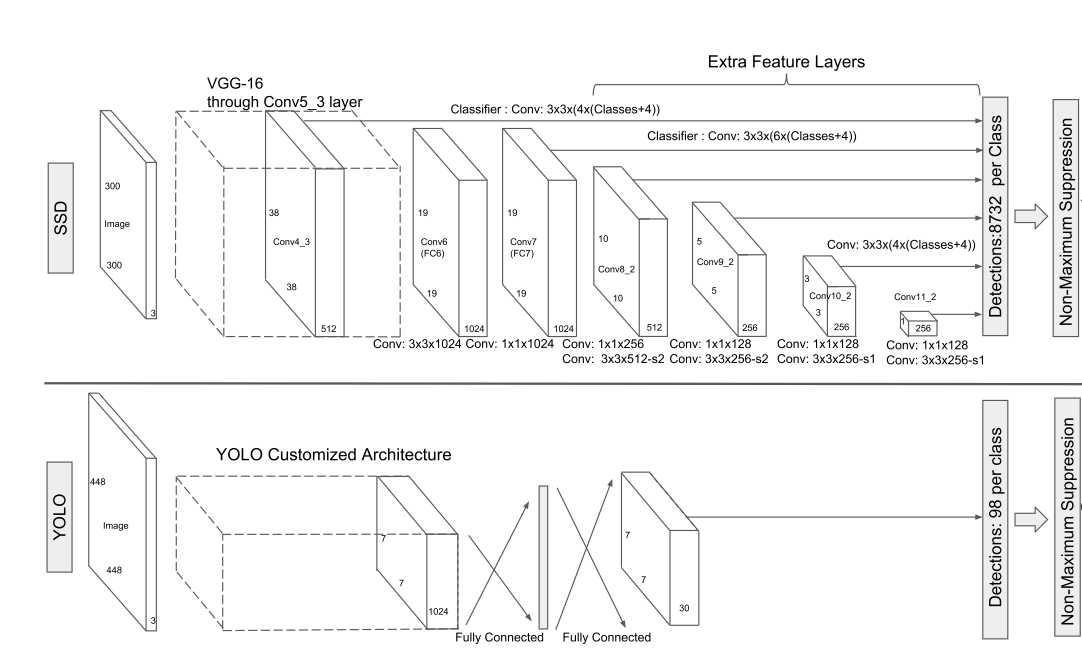
\includegraphics[width=0.9\textwidth]{fig/architecture}
		\caption{Two One Shot Detectors (old) Yolo and SSD \cite{Liu}}
		\label{fig:architecture}
	\end{figure}
	
	\subsection{Basic Concept}
	Single Shot Detectors are (fully) convolutional networks that produce several bounding box predictions in one network evaluation. Predictions are made for a fixed set of \textit{anchor boxes} (also default/prior boxes). Each box resides at a pre-determined location and has a pre-determined size and aspect ratio. The detector predicts "adaptions" to these default coordinates for each of the boxes. Additionally it predicts class confidence scores for each of these boxes. Usually this produces numerous bounding boxes in one evaluation. The predictions are filtered in a final non-maximum-suppression step.
	
	%----------------------------------------------------------------------------------------
	\subsection{Anchor Boxes}
	Usually the image is split in several grid cells. To the center of each grid cell fall several anchor boxes with multiple aspect ratios. This can be seen in \autoref{fig:anchors}.
	
	For SSD the amount/location of anchor boxes is determined by the number of predictor layers. Each predictor layer produces boxes at a certain location/scale. The aspect ratios are selected by hand. 
	
	For Yolo the amount of anchors boxes doesn't depend on the architecture and is chosen via grid size/ number of boxes. Their aspect ratios are determined by a pre-clustering of the ground truth boxes of a dataset.
	\begin{figure}[h]
		\centering
		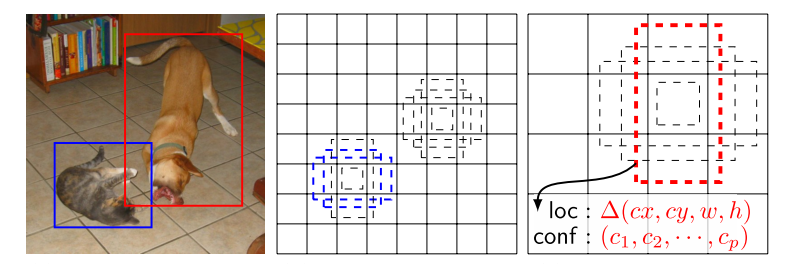
\includegraphics[width=0.9\textwidth]{fig/anchors}
		\caption{Illustration for anchor box concept \cite{Liu}}
		\label{fig:anchors}
	\end{figure}
	%----------------------------------------------------------------------------------------
	\subsection{Architecture}
	
	Usually a classification network like VGG-16 is used as \textit{base network}. On the feature maps of the base network additional convolutional layers are set, that predict class confidences and box coordinates. As for each anchor box a separate output is predicted, each predictor can "specialize" on objects that mostly fall in its aspect ratio/scale/ location (?). The networks implement the final predictions as 1x1 convolutions, thus realizing a fully connected layer more efficiently(?) and allowing various image sizes.
	
	SSD adds several convolutional predictor layers that predict bounding boxes for various scales. They also use one lower layer of the base network for prediction as they assume it preserves more fine grained features.
	
	The first Yolo version as displayed in \autoref{fig:architecture} used a fully connected layer as regression head. However, in the new version they also switched to one convolutional layer.
	
	%----------------------------------------------------------------------------------------
	\subsection{Training Goal}
	SSDs treat object detection as a regression problem. The loss function usually incorporates the aforementioned bounding box coordinates and class scores. During training only one anchor box should be "responsible" for predicting that true box. This responsibility is determined by the location/size of the true box. The SSD paper refers to this as the \textit{matching strategy}.
	
	Yolo matches those boxes to the ones that have their center at a certain grid cell. Among the remaining boxes the one with the highest intersection-over-union (IoU) is chosen. SSD matches anchor and true boxes only based on the IoU.
	
	Yolo Prediction:
	$$t_x,t_y,t_w,t_h,t_o \quad \text{from cell:} c_x, c_y$$
	
	$$x = \sigma(t_x) + c_x \quad y = \sigma(t_y) + c_y \quad w = p_w e^{t_w} \quad h = p_he^{t_h \quad conf = \sigma(t_o)}$$
	where $\sigma(x)$ is softmax function.
	Yolo Loss:\\
	$$ L = \lambda_{coord} \sum_{i=0}^{S^2}\sum_{j=0}^{B} 1^{obj}_{ij}(x_i - \hat{x}_i)^2 + (y_i - \hat{y_i})+$$
	$$
	\lambda_{coord} \sum_{i=0}^{S^2}\sum_{j=0}^{B} 1^{obj}_{ij}(\sqrt{w_i} - \sqrt{\hat{w}_i})^2 + (\sqrt{h_i} - \sqrt{\hat{h}_i})^2 +$$ 
	$$\sum_{i=0}^{S^2}\sum_{j=0}^{B} 1^{obj}_{ij} (C_i - \hat{C_i})^2
	+ 
	\lambda_{noobj} \sum_{i=0}^{S^2}\sum_{j=0}^{B} 1^{noobj}_{ij} (C_i - \hat{C_i})^2
	+ $$$$
	\sum_{i=0}^{S^2}i_i^{obj} \sum_{c \in classes}(p_i(c) - \hat{p_i}(c))^2$$
	
	SSD Loss:\\
	$$L(x,c,l,g) = \frac{1}{N} (L_{conf}(x,c) +\alpha L_{loc}(x,l,g)$$\\
	$$L_{loc}(x,l,g) = \sum_{i \in Pos}\sum_{m \in {cx,cy,w,h}} x_{ij}^k smooth_{L1} (l_i^m - \hat{g}^m_j)$$\\
	$$\hat{g_j}^{cx} = (g_j^{cx} - d_i^{cx})/d_i^{w} \quad \hat{g_j}^{cy} = (g_j^{cy} - d_i^{cy})/d_i^{h}$$\\
	$$\hat{g}_j^w = log(\frac{g_j^w}{d_i^w}) \quad \hat{g}_j^h = log(\frac{g_j^h}{d_i^h})$$
	
	$$L_{conf}(x,c) = - \sum_{i \in Pos}^{N} x_{ij}^p log(\hat{c}_i^p) - \sum_{i \in Neg} log(\hat{c_i}^0) \quad \hat{c_i}^p = \frac{exp(c_i^p)}{\sum_{p} exp(c_i^p)}$$
	\subsubsection{Negatives}
	
	%----------------------------------------------------------------------------------------
	\subsection{Data Augmentation}
	
	\subsection{Comparison}
	\subsubsection{Yolo}
	\begin{enumerate}
		\item Only one convolutional layer for prediction
		\item Anchor boxes determined in pre-clustering step
		\item At most one GT object per grid cell
		\item Assigns GT based on grid cell, at most one GT box per grid cell
	\end{enumerate}
	\subsubsection{SSD}
	\begin{enumerate}
		\item 6 Convolutional layers
		\item Assigns anchor based on iou, several anchors can be responsible for one GT, each GT has at least one anchor
	\end{enumerate}
	
	\subsection{Additional Work on One-Shot-Detectors}
	
	\subsubsection{LCDNet\cite{TripathiSanDiego}}
	
	Aims to bring one shot detection to be runnable on embedded devices.
	
	\begin{itemize}
		\item Quantizies model for inference with 8bit. Records min and max value for each layer and quantizes everything between 0,255
		\item Replaces fully connected layers with convolutional layers
		\item Replaces LeakyRelu with Relu in all but the last (faster?)
		\item Softmax on classification, Sigmoid on confidence
		\item Sigmoid if only one class
		\item quantization mainly effects localization
	\end{itemize}
	
	\subsection{Squeeze Det \cite{Wu}}
		
	\subsection{Summaries}
	\subsubsection{Object Detection}
		\paragraph{Scalable Object Detection using Deep Neural Networks\cite{Erhan}}
		\begin{itemize}
			\item[-] Generates number of bounding boxes as object candidates (class agnostic) and confidences for each box
			\item[-] For each Bounding Box a classifier is run e.g. DNN
			\item[-] Training: If the number of boxes k is larger than the number of objects b, only b boxes are matched while the confidence of the others is minimized
			\item[-] Assignment problem $$F_{match}(x,l) = \frac{1}{2}\sum_{i,j}x_{ij}||l_i - g_j||^2_2$$ where $x_ij$ is one if the ith prediction is assigned to the jth ground truth object
			\item[-] Confidence: 
			$$F_{conf}(x,c) = - \sum_{i,j}x_{ij}*\log(c_i)-\sum_{i}(1-\sum_{j}x_{ij})\log{1-c_j}$$
			\item[-] Speed up training by clustering (kmeans) of ground truth and using it as prior (prior matching)
			\item[-] Can be defined to output boxes only for a particular class by training the bounding boxes on that class
			\item[-] Number of parameters grows linearly with number of classes
			\item[-] Authors argue two step process (region proposal + classification) is better
			\item[-] Architecture based on AlexNet
			\item[-] Predicted boxes are merged using non-maxima surpression
			\item[-] One shot(50\%), +2scales (75\%)
			\item[-] OverFeat/ Selective Search are faster but much more expensive
		\end{itemize}

	\subsubsection{(Re-) Localization}
	\paragraph{PoseNet: A Convolutional Network for Real-Time 6-DOF Camera Relocalization \cite{Kendall}}
	\begin{itemize}
			\item[-] Relocalizes, is trained on images from the scenes where it is applied	\item[-] Accuracy 2m and 3$\degree$  in 50 km$^2$ outdoors, 0.5m and 5$\degree$ indoors, 5ms per frame
		\item[-] ConvNet 23 layers, Image resolution 224x224
		\item[-] transfer learning from recognition/classification datasets (ConvNet is trained on classification tasks)
		\item[-] based on GoogleNet, affine regressors instead of softmax\item[-] automatic training data generation (structure from motion)
		\item[-] learns p from arbitrary global reference frame
		\item[-] $loss(I) = || \hat{x}-x||_2 + \beta*||\hat{q}-\frac{q}{||q||}||_2$
		\item[-] separating position/orientation led to drop in performance
		\item[-] PoseNet evaluation at single center crop + Dense PoseNet 128 uniformly spaced crops (time increase 95ms, only slight accuracy increase)
		\item[-] Training data generated using structure from motion (Cambridge Scene) and 7 Scenes (Microsoft) for indoor

	\end{itemize}
	 \paragraph{A Deep Learning Based 6 Degree-of-Freedom
	 	Localization Method for Endoscopic Capsule Robots \cite{Turan2017}}
	 	\begin{itemize}
	 		\item[-] not published yet?
	 		\item[-] Uses 6-DOF camera pose directly
	 		\item[-] based on GoogleNet (9 Inception modules) trained on ImageNet
	 		\item[-] $loss(I) = ||\hat{x}-x||_2 + ||\hat{q}-q||_2$
	 		\item[-] Dataset of 10 000 frames taken from LM103 - EDG (EsophagoGastroDuodenoscopy) Simulator
	 		\item[-] 0.18cm RMSE on a trajectory of 18cm
	 		\item[-] Although 3 different cameras are used and the frames are separated for training and testing, its still the same "stomach". With 10 000 frames on a trajectory of 18 cm, won't the system just recognize the position?
	 		\item[-] Ground truth determined by seperate cameras 
	 	\end{itemize}
	 	\subsubsection{Object Pose Estimation}
	 	\paragraph{3D generic object categorization localization and pose estimation \cite{Savarese}}
	 	\begin{itemize}
	 		\item[-] Other approaches use different class for different poses
	 		\item[-] Object model is separated in different parts of the object based on different view points (front view)
	 		\item[-] Different parts are connected when another part is visible from the front view via affine transformation
	 		\item[-] Generally such models can't handle inter class variations very good or increase in complexity as number of parts is increased. In this paper this is apparently not the case
	 	\end{itemize}
	 	\paragraph{Uncertainty-Driven 6D Pose Estimation of Objects and Scenes from a Single RGB Image
	 		Eric \cite{Brachmann}}
	 	\begin{itemize}
	 	\item[-] Intermediate representation are object coordinates, continious part labeling that are jointly regressed for every pixel in the image
	 	\item[-] Based on auto context (Classifiers with several stages)
	 	\item[-] (1) (Auto context) Random forest with L1 regularization predicts labels and object coordinates for every pixel (2) Ransac predicts poses from 2d-3d correspondences guided by uncertainty labels
	 	(3) Refinement
	 	\item[-] Random forest predicts (probability to belong to object + 3d coordinate|given belonging to object)
	 	\item[-] Stacked Forests (Auto context) refine output on previous smoothed output (Geodesic Forest). The smoothing is done to enforce coupling of neighbors 
	 	\item[-] RANSAC formulates hypothesis by drawing 4 correspondences and solving PnP
	 	\item[-] Outperforms PoseNet in indoor localization
	 	\item[-] 6D within 5cm and 5 degree only 40 \% (With RGB-D 82.5\%), on other set 50 \% with unknown scene average median error 8.5cm 3.3°
	 	\item[-] Biggest translational error in z direction
	 	\item[-] Multi object detection/pose estimation in 1-4 seconds, not optimized, most time spend in searching for object hypothesis
	 	\end{itemize}
	 	\paragraph{A Comparative Analysis and Study of Multiview CNN Models for Joint Object Categorization and Pose Estimation\cite{Elhoseiny}}
	 	\begin{itemize}
	 		\item[-] While detection needs pose invariant features, pose estimation needs the pose
		 	\item[-] Single instance 3d model
		 	\item[-] Discrete pose approaches (pose as classification)
		 	\item[-] Trains pose regressor and classifier on output of different levels to measure quality of features
		 	\item[-] Later layers "forget" about pose, paper suggests early branching
	 	\end{itemize}
	\subsubsection{Other}
		 \paragraph{Deformable Convolutional Networks \cite{Dai}}
		 \begin{itemize}
		 	\item[-] Addresses problem of modeling geometric transformations
		 	\item[-] Introduces \textit{Deformable Convolution} which adds 2D offsets to the regular sampling grid. The offsets are learned from the data.
		 	\item[-] Introduces \textit{Deformable RoI pooling} which adds offsets to bins of pooling layers. The offsets are also learned from the data.
		 	\item[-] Further alternatives to have more variable feature maps: Spatial Transformer Networks, Active Convolution, Effective Receptive Field, Atrous Convolution, DeepID-Net, Spatial manipulation in RoI pooling (handcrafted), DPM (handcrafted)
		 	\item[-] Light-weight version of STN, easier to train and to integrate
		 	\item[-] Receptive fields seem to scale with the size of objects
		 	\item[-] Model complexity is increased by only 1-2%
		 	\end{itemize}
		 	

\begin{landscape}

\begin{table}[]
	
	\caption{Object Detection}
	\label{my-label}
	\begin{tabular}{|p{3cm}|p{3cm}|p{3cm}|p{3cm}|p{3cm}|p{3cm}|p{3cm}|p{3cm}|}
		\hline
		& \multicolumn{3}{l|}{Traditional} & \multicolumn{4}{l|}{Deep}   \\ \hline
		& Viola\&Jones    				   & HoG    & DPM   		   & R-CNN    & YOLO         & SSD & OverFeat \\ \hline
		Feature Detector & Haar					   & HoG    & Multiple Hogs and virtual springs   & Learned by CNN     &  Learned by CNN            & & \\ \hline
		Detection & \multicolumn{3}{l|}{Sliding Window, high filter responses indicate there is an object} & NN in sliding window detects regions for possible objects, For each proposed region a classification is run & Image is split in Grid each Grid spawns Bounding boxes and gives class probabilities & & \\
		\hline
		Accuracy (voc) &  & & & 73.2 mAP & 63.4 mAP & 74.3 mAP & \\ 
		\hline
		Speed & & & & 7 FPS (Faster-RCNN) & 45 FPS & 59 FPS & \\
		\hline
		Strengths & & & & & &  &\\
		\hline
		Weaknesses & & & & & &  &\\
		\hline
		\end{tabular}
		
		\end{table}
		\end{landscape}	
		\bibliographystyle{abbrv}
\bibliography{literature.bib}


\end{document}
